% ====================================================================
%+
% SECTION:
%    SolarSystem_OrbitalAccuracy.tex
%
% CHAPTER:
%    solarsystem.tex
%
% ELEVATOR PITCH:
%    How secure is the orbit - is it going to hit us?
%    Libration amplitude distribution for TNOs?
%    Can we find it after X years for further study?
%    Can we identify the source region for NEOs within the main belt?
%-
% ====================================================================

\section{Orbital Accuracy}
\def\secname{\chpname:orbits}\label{sec:\secname}

A vast number of moving objects will appear in LSST images. Multiple
observations of a common object will be linked, and a preliminary orbit
derived. However, the orbital elements (semi-major axis, eccentricity,
etc.) will have some uncertainty. Short arcs --- that is, a small amount
of time between the first and last observation of a given object ---
produce orbits with large uncertainties on the orbital elements. As arc
length grows, the orbital uncertainties decrease.

A number of science cases require relatively small uncertainties on
orbital elements. Perhaps most importantly, small uncertainties can aid
in discriminating between Near Earth Objects that might and might not
impact the Earth. A more subtle example relates to the libration
amplitude distribution for TNOs, which can be compared to predictions
from Solar System formation models. Only with small uncertainties on
orbital elements can the libration amplitudes be determined to
sufficient precision to compare to the predictive models. Finally,
during and after the primary LSST survey additional measurements will be
desired for further characterization of many objects. Only if the
orbital elements are sufficiently well know can objects be studied later
with other facilities. For example, to carry out spectroscopy, the
position of the object must be known to approximately 1~arcsec (the
width of a typical slit). This places strong requirements on the
knowledge of the orbital elements.


% --------------------------------------------------------------------

\subsection{Target measurements and discoveries}
\label{sec:\secname:targets}

The relevant data here are positions as a function of time for a given
object (assuming that the linking of measurements to a given object is
satisfactory). Assuming that the accuracy and precision of each
measurement are approximately constant (likely, since all will be made
by the same observing system), the only significant factor that improves
the knowledge of the orbit is extending the observational arc. The
observing strategy employed by LSST must therefore have a cadence in
which objects are revisited with the largest possible arcs that still
allow linking of observations. In other words, if the observations of a
given object are too widely spaced, linking may not be possible, so,
even though the arc is long, the linking is poor and the object yield is
low. If the observations are made too densely in time, linking is likely
to be good, but the arc may not be very long. A middle ground is
desired.

% --------------------------------------------------------------------

\subsection{Metrics}
\label{sec:\secname:metrics}

The best metric here would be to take the actual series of observations
of each object, add appropriate astrometric noise to each observation
according to its SNR, cull observations which would not be `linkable' to
the rest (i.e. observations which occur on a single night far from other
nights in the arc, or even a series of observations which occur too many
years away from other observations of the same object), and then fit an
orbit to the remaining observations and determine the uncertainty in its
parameters. This is work for the future however; our first simple proxy
uses the {\tt ObsArcMetric} to just look at the time between the first
and last observation of an object. For many objects, this will be fairly
close to the actual arc length of the linkable observations, as most
objects receive many observations clumped together when they are
observable, so this simple proxy makes a reasonable starting point.


% --------------------------------------------------------------------

\subsection{OpSim Analysis}
\label{sec:\secname:analysis}

\begin{figure}
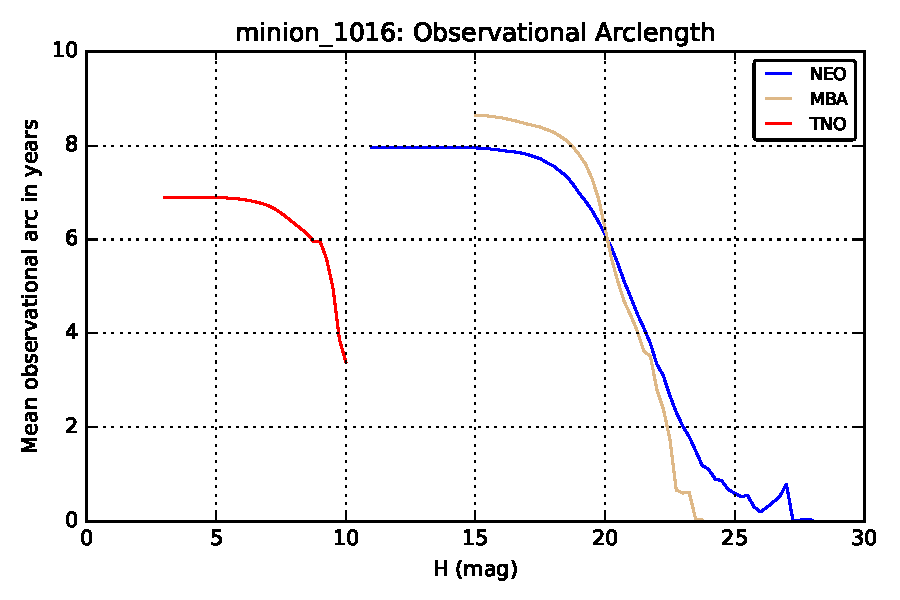
\includegraphics[width=6in]{figs/solarsystem/minion_1016_ObsArc_neo_tno_mba_MOOB_ComboMetricVsH}
\caption{Mean observational arc length, in years, for NEO, MBA and TNO
  populations as a function of $H$ magnitude.
\label{obsarc}}
\end{figure}

In \opsimdbref{db:baseCadence}, the mean observational arc length for
NEOs and MBAs is about 8~years for bodies larger than 1~km, and about
6~years for 300~m bodies. With these
orbital arcs, the orbits will be quite well known,
% xxx quantify -- how well! xxx,
meaning that the majority
of LSST-observed objects will have orbits that are sufficiently
well known that the above science cases can be carried out.
In some special cases --- for example, the case where
an NEO's orbit still presents a signficant probability
of terrestrial impact --- additional non-LSST follow-up
may be needed, but this will be a small minority of cases.

% xxx what we probably want is fraction of objects
% with arcs longer than 3 years (say) as a fxn of
% H mag, for NEOs/MBAs/TNOs. xxx

% --------------------------------------------------------------------

\subsection{Discussion}
\label{sec:\secname:discussion}

The simple proxy metric above should be improved to account for
potential difficulties in linking observations, and to include actual
orbital fitting to determine orbital uncertainties. The timing of
observations effects the final orbital accuracy significantly,
particularly for TNOs, and having a good distribution on the times of
observations can improve orbital accuracy more quickly than would
naively be expected from a simple observational arclength scaling.

A figure of merit, including requirements on the orbital accuracy for
various classes of objects, should also be developed.

% --------------------------------------------------------------------

\navigationbar
